\begin{figure*}[ht]
  \centering
  \begin{subfigure}[c]{0.36\textwidth}
    \centering
    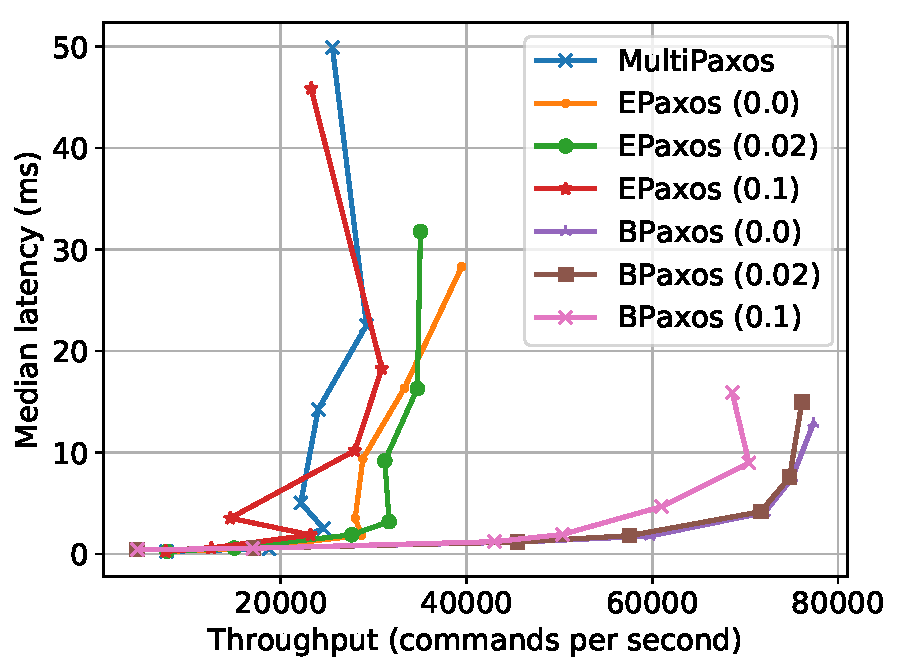
\includegraphics[width=\textwidth]{assets/nsdi_fig1_lt_f1.pdf}
    \caption{
      Latency-throughput curves for Multipaxos, EPaxos, and BPaxos. EPaxos and
      BPaxos are run with 0\%, 2\% and 10\% conflict rates. Here, $f = 1$.
    }\figlabel{EvalLtF1}
  \end{subfigure}
  \begin{subfigure}[c]{0.36\textwidth}
    \centering
    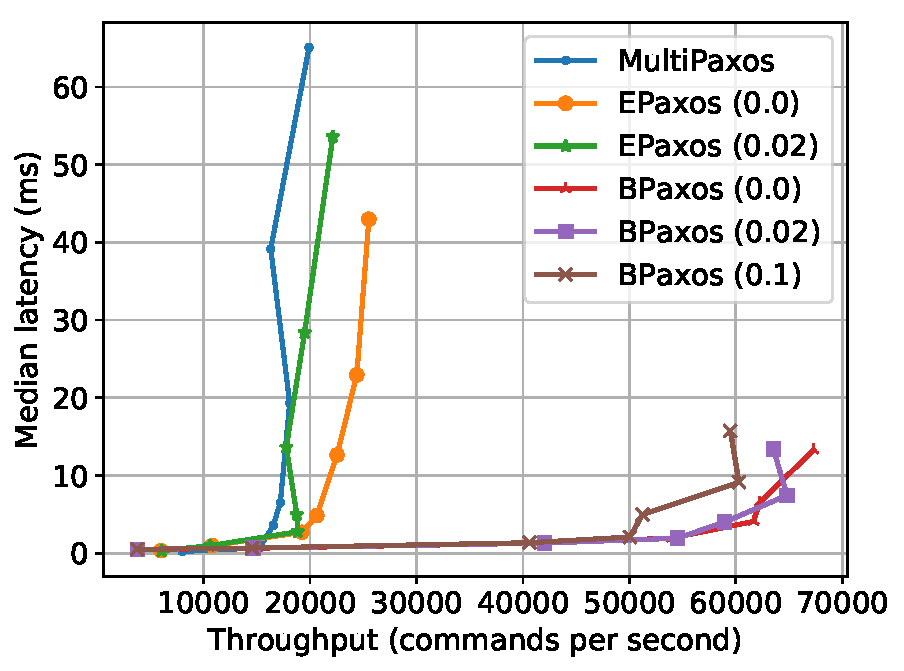
\includegraphics[width=\textwidth]{assets/nsdi_fig1_lt_f2.pdf}
    \caption{The same as \figref{EvalLtF1} but with $f=2$.}%
    \figlabel{EvalLtF2}
  \end{subfigure}
  \begin{subfigure}[c]{0.23\textwidth}
    \centering
    \small
    \begin{tabular}{lccc}
      \toprule
      \multicolumn{1}{c}{Protocol} &
      \multicolumn{3}{c}{Number of clients} \\
      %
                    & 1    & 10   & 50 \\\midrule
      Multipaxos    & 0.24 & 0.52 & 2.49 \\
      EPaxos (0.0)  & 0.25 & 0.56 & 1.83 \\
      EPaxos (0.02) & 0.25 & 0.57 & 1.89 \\
      EPaxos (0.1)  & 0.25 & 0.58 & 1.87 \\
      BPaxos (0.0)  & 0.41 & 0.56 & 1.16 \\
      BPaxos (0.02) & 0.41 & 0.56 & 1.17 \\
      BPaxos (0.1)  & 0.41 & 0.55 & 1.21 \\
      \bottomrule
    \end{tabular}
    \caption{%
      Median latency values (ms) from \figref{EvalLtF1}.
    }\figlabel{EvalLtTable}
  \end{subfigure}
  \caption{%
    Latency and throughput of Multipaxos, EPaxos, and BPaxos for varying number
    of clients, conflict rates, and values of $f$. Data is shown for $1$, $10$,
    $50$, $100$, $300$, $600$, and $1200$ clients.
  }\figlabel{EvalLt}
\end{figure*}
